%If you start a line with a "percent" symbol (like %), then that line is a "comment" and won't show up in your actual document.  

%Every document starts with a documentclass. 
\documentclass[11pt]{article}

%After that, it's useful to list an author and give a title.
\author{William Fu}
\title{Problem Set 1}

%Graphicx is used to include pictures in LaTeX files. 
\usepackage{graphicx}

%The AMS packages. They contain a lot of useful math-related goodies.
\usepackage{amsthm}
\usepackage{amsmath}
\usepackage{amsfonts}

\usepackage[sexy]{evan}
\begin{document}

\section{Distributions}
\begin{example}[Distribution of Angles]
If $x_1$ is uniformly selected from $S^{N-1}$ (the sphere in dimension $N$), then the angle between the randomly chosen vector and another, $\rho(\xi, x_1)$ will be around $O(1/\sqrt{N})$. 
\end{example}
Justification: Without loss of generality, let
\[ \xi = e_1 = [1, 0, \dots]^T\]
To generate a random direction, we will first generate a random matrix and normalize.
\[ y_1, \dots, y_n ~ \mathcal{N}(0, 1)\]
\[ x_i = \frac{y_i}{\sqrt{\sum y_i^2}}\]
\[ x = [x_1, \dots, x_n]^T\]
Then, we can directly calculate the angle $\rho$ between $\xi$ and $x$.
\[ \rho(e_1, x) = \frac{y_1}{\sqrt{\sum y_i^2}} = \frac{y_1/\sqrt{N}}{\sqrt{\sum y_i^2/N}}\]
Note that the denominator goes to 1. Then, as we take the large $N$ case, we see that
\[ \rho(x, \xi) ~ O(\frac{1}{\sqrt{N}}\]
We can see this phenomenon numerically very well once we start getting to $N=1024$.

\section{Gibbs Distribution and Optimization}

Let $x = (x_1, \dots, x_N)$, and $H(x) = H(x_1, \dots, x_N)$. We want to investigate the value
\[ \min\left( \frac{H(x)}{N} \right)\]
The best tool that we will use is the Gibbs distribution,
\[ P_g(x) = \frac{e^{-\beta H(x)}}{ Z(\beta)}\]
$\beta \ge 0$ is the inverse temperature and serves as a smooth interpolation between $\beta=0$ and $\beta = \infty$ case. The definition of free energy is
\begin{equation*}
	F(\beta) = -\frac{1}{\beta}\log Z(\beta)
\end{equation*}
We showed last time that taking the limit,
\begin{align*}
	\lim_{\beta \to \infty} F(\beta) = \min_x H(x)
\end{align*}

\subsection{Important Properties}
\begin{enumerate}
	\item The limit of free energy.
		\[\lim_{\beta \to 0} F(\beta) = \min_x H(x)\]


	\item Bracket Notation
		\[ \langle H(x) \rangle = \sum_x H(x) P_G(x) = \frac{\sum_x H(x) e^{-\beta H(x) }}{Z(\beta)}\]
	
	\item Expectation of Hamiltonian
		\[ \frac{d}{d \beta} (-\beta F(\beta)) = \langle H(x) \rangle \]

	\item Shannon Entropy
		\[ F(\beta) = \langle H(x) \rangle - \frac{1}{\beta}S(P_G(x))\]

\item  Another Shannon Entropy
	\[ S(P_G(x)) = \beta^2 \frac{d}{d \beta} F(\beta)\]
\end{enumerate}


\subsection{Ideas about the Entropy}

	Suppose that $x \in \{\pm 1\}^N$. Then, let's say that the energy levels for this system go to $M$ discrete energy levels.
	\[ \frac{H(x)}{N} \in \{E_1, E_2, \dots, E_M\}\]
Let $\Omega$ be the number of configurations that go to each energy level,
\[ \Omega(E_i) = |\{ x ~ | ~ \frac{H(x)}{N} = E_i\}|\]
Since we started out with $2^N$ states, we expect that $S(E_i)$ will be exponential. 
Therefore, we will use a log definition and call it $S$, 
\[ S(E_i) = \frac{1}{N} \log |\{ x ~ | ~ \frac{H(x)}{N} = E_i\}|\]
We can now define our probability distribution as
\[ P_G(x) = \frac{e^{-\beta H(x)}}{Z(\beta)} \]
Let's draw a sample, $x^* ~ P_G(x)$. 

\begin{example}[Dominance of Energy State]
	If we draw a sample $x^* ~ P_G(x)$, as $N \gg 1$, the probability of getting a specific energy level is very high.
\end{example}

We can directly compute this. by trying to calculate the probability.
\begin{align*}
P(H(x^*) = E_i) 
&= \frac{e^{-\beta E_i}}{Z(\beta)} \cdot (\text{ size of set } E_i) \\
&= \frac{e^{-\beta E_i} e^{NS(E_i)}}{\sum_{j=1}^M e^{-\beta E_j N} e^{NS(E_j)}}
\end{align*}
We can see that we have a factor of $N$ in both terms in the distribution. Note that in the general case, when we have this pattern and $N \gg 1$, 
\begin{equation*}
	\frac{e^{N \theta_1}}{ e^{N \theta_1} + e^{N \theta_2} + \cdots + e^{N \theta_m} } \approx 1 ~ ~ ~ ~ ~ ~ ~ \text{ if } \theta_1 = \max(\theta_i)
\end{equation*}
Likewise, the term will go to zero if the $\theta$ on the top is not the largest value. Therefore, applying this to our original problem, we can use the substitution $\theta_i = S(e_i) - \beta E_i$. Therefore, only the cluster that maximizes $\theta$ will have probability $P_G(E_{\max}) \approx 1$, while all of the other clusters will have around probability $P_G(E_i) \approx 0$. 
Therefore, since all of the particles are clustered around one energy level, the Shannon entropy will just be $S(E_{\max})$ in the large $N$ limit. Furthermore, the free energy in this case is 
\begin{align*}
	- \frac{1}{\beta} \log Z(\beta)
	&= -\frac{1}{\beta N} \log\left( e^{-\beta N E_{\max}} e^{N S(E_{\max})} \right) \\
	&= E_{\max} - \frac{1}{\beta}S(E_{\max})
\end{align*}

















\section{The 1D Ising Model}
We have particles with different spins, all attached on a line.

\begin{center}
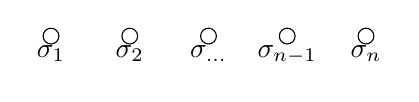
\begin{tikzpicture}
	\draw (0, 0) circle[radius=0.1] node[below] {$\sigma_1$};
	\draw (1, 0) circle[radius=0.1] node[below] {$\sigma_2$};
	\draw (2, 0) circle[radius=0.1] node[below] {$\sigma_{\dots}$};
	\draw (3, 0) circle[radius=0.1] node[below] {$\sigma_{n-1}$};
	\draw (4, 0) circle[radius=0.1] node[below] {$\sigma_n$};
\end{tikzpicture}
\end{center}

We will have the interactions between only the adjacent particles.
\[H(\sigma) = -\sum_{i=1}^{N-1} \sigma_i \sigma_{i+1} ~ ~ ~ ~ ~ ~ ~ ~ \sigma \in \{\pm 1\}\]
\[ P_G(\sigma) = \frac{e^{-\beta H(\sigma)}}{Z(\beta)}\]
Then, the partition function will be the sum of $2^N$ states of the particles.
\[ Z(\beta) = \sum_{\sigma_1, \dots, \sigma_n \in \{\pm 1\}} \exp\left( e^{ \beta \sum \sigma_i \sigma_{i+1}} \right)\]
We can find a closed form solution using two different methods. We can either use recursion on $N$ to find a closed form solution. 
\end{document}
